%\documentclass{article}
%\usepackage[utf8]{inputenc}
%\usepackage{tikz}
%\usetikzlibrary{positioning}

%\begin{document}
	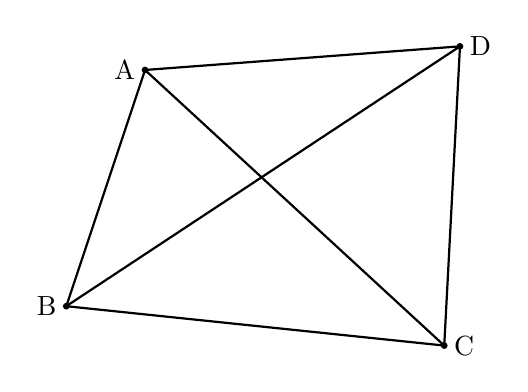
\begin{tikzpicture}
		\draw[black, thick] (0,0) --(1.0001,3); 
		\filldraw[black] (0,0) circle (1pt) node[anchor=east] {B}; 
		\draw[black, thick] (1.0001,3)--(5,3.3);
		\filldraw[black] (1.0001,3) circle (1pt) node[anchor=east] {A};
		\draw[black, thick] (5,3.3)--(4.8,-0.5);
		\filldraw[black] (5,3.3) circle (1pt) node[anchor=west] {D};
		\draw[black, thick] (4.8,-0.5)--(0,0);
		\filldraw[black] (4.8,-0.5) circle (1pt) node[anchor=west] {C};
		\draw[black, thick] (5,3.3)--(0,0);
		\draw[black, thick] (1.0001,3)--(4.8,-0.5);
	\end{tikzpicture}


%\end{document}